\documentclass[../main.tex]{subfiles}

\begin{document} %%%%%%%%%%%%%%%%%%%%%%%%%%%%%%%%%%%%%%%%%%%%%%%%%%%%%%%%%%%%
\section{TDA conjunto} 
    \subsection{Árbol binario AB}
        Un árbol binario es una estructura de datos que relaciona información de manera jerárquica no lineal, con un nodo raíz y dos subárboles disjuntos, llamados izquierdo y derecho. Cada nodo puede tener, a lo sumo, dos hijos, y el grado de un árbol binario es el mayor grado de cualquiera de sus nodos.\\

        \underline{Algunas de las características de un árbol binario son:}
        \begin{itemize}
            \item La \textbf{raíz} es el primer nodo del árbol y no tiene padre.
            \item Los nodos hoja son los nodos que no tienen hijos.
            \item Los nodos internos son los nodos que tienen al menos un hijo.
            \item El subárbol izquierdo de un nodo es el árbol formado por su hijo izquierdo y todos sus descendientes.
            \item El subárbol derecho de un nodo es el árbol formado por su hijo derecho y todos sus descendientes.
            \item La altura de un nodo es la longitud del camino más largo desde el nodo hasta una hoja.
            \item La profundidad de un nodo es la longitud del camino desde la raíz hasta el nodo.
            \item El nivel de un nodo es su profundidad más uno.
            \item La altura de un árbol es la altura de su raíz.
            \item El orden de un árbol binario es el número total de nodos que tiene.
        \end{itemize}

        \paragraph{Tipos de árboles binarios:}
        Un árbol binario es un árbol en el que ningún nodo puede tener más de dos subárboles. En un árbol binario cada nodo puede tener cero, uno o dos hijos (subárboles). Se conoce el nodo de la izquierda como hijo izquierdo y el nodo de la derecha como hijo derecho.

        \begin{itemize}
            \item \textbf{Árbol binario de búsqueda:} Es un árbol binario que cumple con la propiedad de que para cada nodo, el valor de todos los nodos del subárbol izquierdo es menor o igual al valor del nodo y el valor de todos los nodos del subárbol derecho es mayor o igual al valor del nodo.
        \end{itemize}
        
        La diferencia entre un árbol binario y uno de búsqueda es que el primero no tiene ningún orden específico para organizar los elementos, mientras que el segundo sí lo tiene. Un árbol binario puede tener cualquier forma y distribución de los nodos, siempre que cada uno tenga como máximo dos hijos. Un árbol binario de búsqueda tiene una forma y distribución determinadas por la relación de orden entre los elementos.

        % Cargamos la imagen
        \begin{figure}[ht]
            \centering
            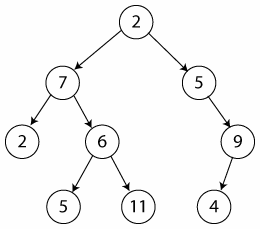
\includegraphics[width=0.3\textwidth]{images/arboles/arbol_binario.png}
            \caption{Árbol binario} 
        \end{figure}

        La única condición que debe cumplir un árbol binario es que cada nodo puede tener como máximo dos hijos. No hay ninguna restricción sobre el orden de los elementos, ni sobre la forma del árbol.\\

    \subsection{Árbol binario de búsqueda ABB}
        Un árbol binario de búsqueda también llamado BST (acrónimo del inglés Binary Search Tree) es un tipo particular de árbol binario que presenta una estructura de datos en forma de árbol.

        % Cargamos la imagen
        \begin{figure}[ht]
            \centering
            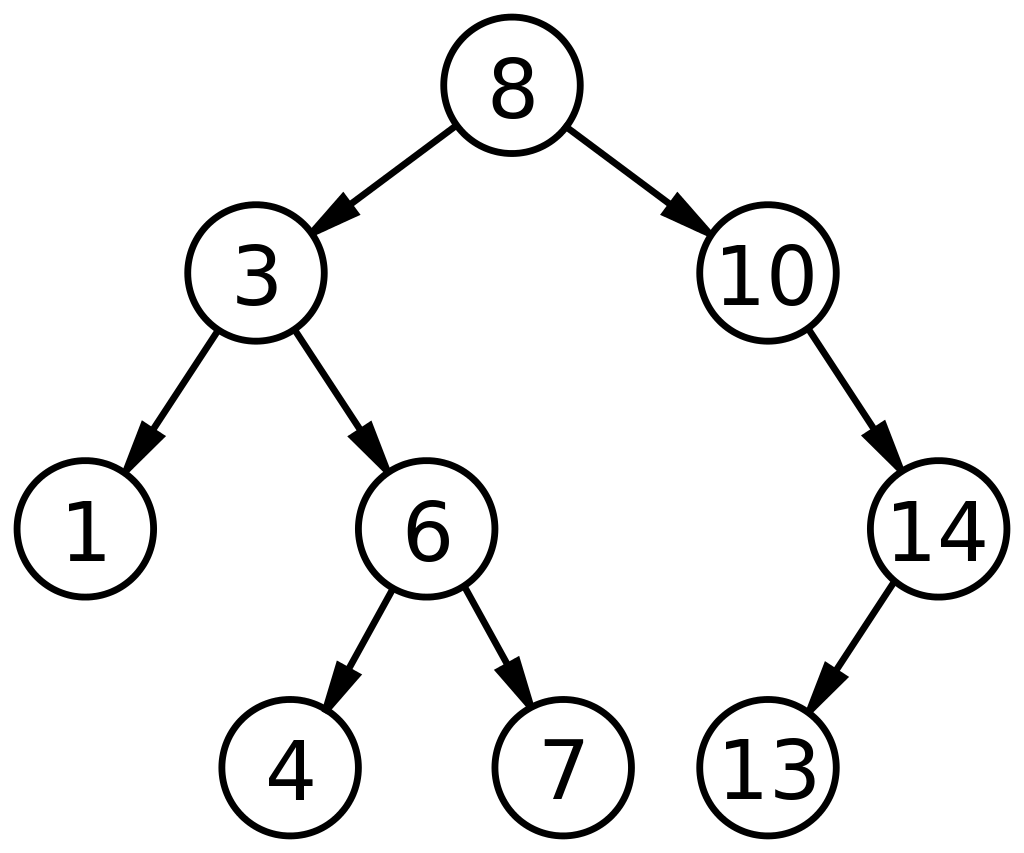
\includegraphics[width=0.3\textwidth]{images/arboles/ABB.png}
            \caption{Árbol binario de búsqueda} 
        \end{figure}
        
        \subsubsection{Propiedad de ABB:} 
            Un ABB es un AB donde (esto es lo que lo diferencia de un AB común):
            \begin{itemize}
                \item El hijo izquierdo, y todos sus hijos, son menores que la raíz.
                \item El hijo derecho, y todos sus hijos, son mayores que la raíz.
            \end{itemize}


        \subsubsection{Operaciones}
            \begin{itemize}
                \item \textbf{Insertar:} Inserta un elemento en el árbol.
                \item \textbf{Eliminar:} Elimina un elemento del árbol.
                \item \textbf{Buscar:} Busca un elemento en el árbol.
                \item \textbf{Recorridos:} Recorre el árbol en distintos órdenes.
            \end{itemize}

        \subsubsection{Insertar} 
            Los ABB crecen “de arriba hacia abajo”, es decir que se genera un nodo cuando se encuentra nulo el puntero apropiado.
        
        \subsubsection{Eliminar o Borrado} 
            Casos Posibles \cite{ABB-Eliminar_nodos} :
            \begin{enumerate}
                \item \textbf{Nodo hoja:} Se elimina el nodo y se pone a nulo el puntero del padre.
                \item \textbf{Nodo con un hijo:} Se elimina el nodo y se pone a nulo el puntero del padre. El hijo pasa a ser hijo del padre del nodo eliminado.
                \item \textbf{Nodo con dos hijos:} 
            \end{enumerate}

            \underline{Caso 3: Eliminar nodo con dos hijos.}
            \begin{enumerate}
                \item Localizar el nodo predecesor o sucesor del nodo a eliminar.
                    \begin{itemize}
                        \item predecesor es “el mayor de los menores”
                        \item sucesor es “el menor de los mayores”
                        \item Para la implemtacion es igual de eficiente usar uno u otro.
                    \end{itemize}
                \item El valor del predecesor (o sucesor) se copia en el nodo a eliminar.
                \item Eliminar el nodo del predecesor (o sucesor).
            \end{enumerate}

        \subsubsection{Busqueda} 
            Debemos comenzar por el nodo raíz e ir descendiendo a izquierda o derecha, ya sea que el valor que estemos buscando sea menor o mayor que el dato del nodo que estemos comparando

        \subsubsection{Recorridos} 
            Los recorridos se clasifican en dos categorías. Video YouTube \cite{ABB-Recorridos_youtube}:
            \begin{itemize}
                \item Profundidad: En los recorridos en profundidad se procesa cada nodo, su subárbol izquierdo y el derecho. Se usa una Pila.
                    \begin{itemize}
                        \item Preorden. $\Theta(n)$
                        \item Inorder $\Theta(n)$
                        \item Postorder $\Theta(n)$
                    \end{itemize}
                \item Anchura o por niveles $\Theta(n)$: En los recorridos en anchura se procesa cada nodo por niveles. Se usa una Cola.
            \end{itemize} 
        
    \subsection{Arboles balanceados}
        Tipos de árboles balanceados:
        \begin{itemize}
            \item ABB balanceado por su altura.
            \item ABB balanceado por el peso.
        \end{itemize}

        \subsubsection{ABB balanceado por su altura}
            Un árbol binario está balanceado por su altura con diferencia permitida d sii para todo nodo x del árbol se verifica:

            \begin{equation}
                |h_{izq}(x) - h_{der}(x)| \leq d
            \end{equation}

        \subsubsection{ABB balanceado por el peso}
            Un árbol binario está balanceado por su peso con diferencia permitida d sii para todo nodo x del árbol se verifica:

            \begin{equation}
                |peso_{izq}(x) - peso_{der}(x)| \leq d
            \end{equation}

    \subsection{Árboles AVL}
        Los árboles AVL se balancean por altura. Se trata de un tipo de árbol binario de búsqueda que cumple la propiedad de que para cada nodo, la diferencia entre la altura de su subárbol izquierdo y el de su subárbol derecho es como máximo 1.
        
        Se agrega un atributo al nodo que es el factor de balanceo (FB). Este factor tiene tres valores permitidos: 0, 1 o -1, en cualquier otro caso se necesita rebalancear.

        % Cargamos la imagen
        \begin{figure}[ht]
            \centering
            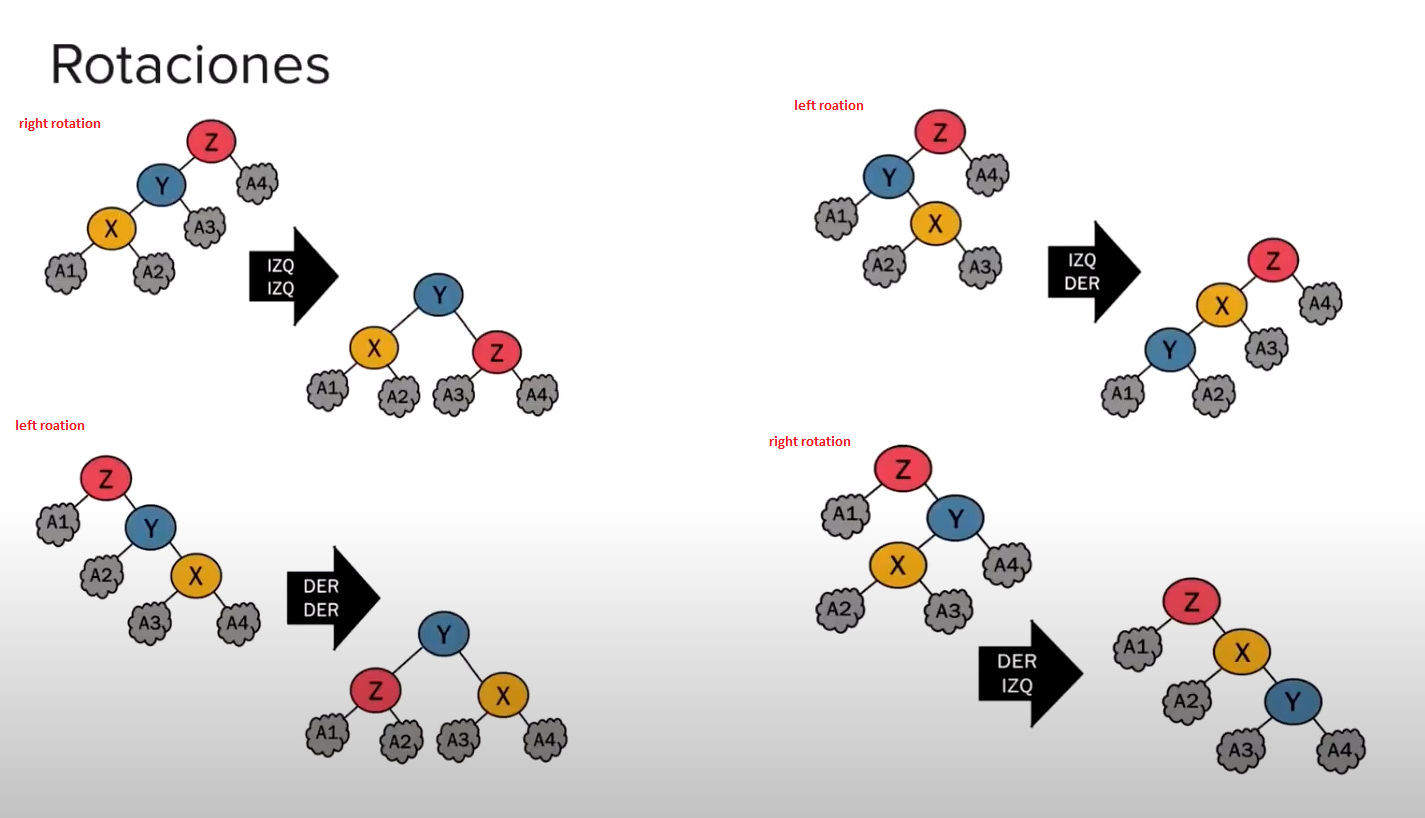
\includegraphics[width=1\textwidth]{images/Rotaciones.png}
            \caption{Rotaciones Árbol AVL}
            \label{fig:AVL} 
        \end{figure}
        
    \newpage

    \subsection{Árboles multivía o de m vías}
        Estas estructuras mejoran la eficiencia del almacenamiento habilitando la posibilidad de tener varios datos o claves en el mismo nodo.
        
        Las claves siempre estarán ordenadas de forma creciente y de manera contigua, es decir que dos claves no puede haber nunca espacio no utilizado. No hay “posiciones vacías” entre dos claves.

        Un árbol de m vías está formado por nodos que pueden contener hasta m-1 claves $(k_0, k_1,k_2, ... , k_{m-2})$.\\

        \underline{Las condiciones que verifica esta estructura son:}
        \begin{enumerate}
            \item Cada nodo tiene $m$ vías (eventualmente pueden estar nulas) y m-1 lugares para almacenar claves.
            \item Las claves (o datos) se almacenan de forma creciente y de manera contigua.
            \item Las claves de los subárboles que están a la izquierda de la iésima clave son menores que la iesima clave.
            \item Las claves de los subárboles que están a la derecha de la iésima clave son mayores que la iesima clave.
            \item No esta balanceado.
        \end{enumerate}

    \subsection{Árbol B}
        Se trata de un árbol de m vías balanceado. Las primaras cuatro condiciones representan un árbol de m-vias.Video YouTube \cite{Árboles-B_youtube}\\

        \underline{Las condiciones que verifica esta estructura son:}
        \begin{enumerate}
            \item Cada nodo tiene $m$ vías (eventualmente pueden estar nulas) y m-1 lugares para almacenar claves.
            \item Las claves (o datos) se almacenan de forma creciente y de manera contigua.
            \item Las claves de los subárboles que están a la izquierda de la iésima clave son menores que la iesima clave.
            \item Las claves de los subárboles que están a la derecha de la iésima clave son mayores que la iesima clave.
            \item Esta balanceado.
            \item Todos los nodos excepto la raíz están completos con claves al menos hasta la mitad.
            \item La raíz, o bien es hoja, o bien tiene al menos dos hijos.
            \item Si un nodo tiene $h$ claves almacenadas, entonces tiene $h+1$ hijos (salvo la raíz y las hojas).
            \item Todas las hojas están en el mismo nivel.
        \end{enumerate}

        \subsubsection{Borrado}
            \underline{Borrado en un árbol B:}
            \begin{itemize}
                \item En hojas: normalmente.
                \item Nodos internos: buscar reemplazante (similar ABB).
                \item Puede haber underflow (nodo con menos claves de las permitidas).
            \end{itemize}

            \underline{Borrado con Underflow:}
            \begin{itemize}
                \item \textbf{Prestar:} Si un hermano tiene más claves de las permitidas, se le puede pedir prestado.
                \item \textbf{Fusionar:} Si un hermano tiene la mínima cantidad de claves, se fusionan los dos nodos.
            \end{itemize}

    \subsection{Estructura B+}
        Cuando es necesario acceder de manera secuencial a los datos almacenados en una estructura de arbol B, puede adicionarse una lista ligada con esos datos, la cual es accessible desde los nodos hoja.\\
        
        \underline{Las condiciones que verifica esta estructura son:}
        \begin{itemize}
            \item Las mismas condiciones que un árbol B.
            \item Todos los datos se almacenan únicamente en los nodos hoja.
            \item Los nodos hoja se encuentran unidos entre sí como una lista enlazada para permitir principalmente recuperación en rango mediante búsqueda secuencial.
        \end{itemize}
        



    

\end{document}  %%%%%%%%%%%%%%%%%%%%%%%%%%%%%%%%%%%%%%%%%%%%%%%%%%%%%%%%%%%%%